\chapter{Chisel-CRV}\label{chiselcrv}
During the project, the author decided to stop the development of F-CSP because
the core decisions to use internal types and rewrite an entirely new
``functional" constraint satisfaction solver were not the right choices in this
context. While researching for an appropriate Java counterpart of F-CSP, three
main options were considered, Choco-Solver \cite{prudchoco4}, Jacop
\cite{online:jacop}, OptaPlanner \cite{online:optaplanner}. These three
libraries offer a solid set of primitives for constraint programming, are
open-source, and are already adopted by a large userbase. After experimenting
with all three libraries, the author decided to use JaCoP as a starting point,
given its flexibility and simplicity compared to the other two.

\section{Jacop}
JaCoP \cite{online:jacop} the acronym for Java Constraint Programming is an
open-source constraint programming solver written in Java. The first release was
published in 2001, and it is still continuously developed. At the time of
writing, its last release, published the 16 November 2020, is version 4.8.0.
Despite being implemented in a high-level language like Java, JaCoP is very
efficient, and it has received many different awards in various constraint
programming competitions. By default, JaCoP comes bundled with a small Scala DSL
for defining constraint, which was the main inspiration for implementing the
Chisel-CRV library.

\par Listing \ref{listing:crv:jacop:alu} is an example on how to declare a
constraint satisfaction problem in JaCoP. At the heart of JaCoP is the class
\mints{Store} (line 8). As the name says, the Store class is used to store all
the current constraints that apply to the problem variables. Thus each variable
must be initialized with a specific \mints{Store} (line 10 - 12). Every variable
has a name and a domain. If no name is given to the variable during its
instantiation, a default name is automatically given to it, and the same goes
for the domain. Each of the variables needs to be saved in a list of variables
and used in combination with the \mints{Store} to solve the current problem.
After having declared the \mints{Store} and the variables, constraints can be
added to the \mints{Store} by invoking its method \mints{impose} and passing as
argument the constraint (line 14 - 21). It is important to note that variables
defined with the \mints{tmp} keyword (line 14, 17, 18) are auxiliary variables
needed to express the constraint. For example, the variable \mints{tmpSum} is a
variable that is equal to the sum of \mints{a} and \mints{b}. This auxiliary
variable is then constrained to have values that are less than 255. When the
problem is defined, it is necessary to create an inference selector by
specifying a \mints{SelectChoicePoint} inference class. This class can be
customized by selecting the type of inference and the ``value-ordering."
Finally, it is possible to declare the depth-first-search method and find a
solution to the problem (line 29).

\begin{code}
\begin{minted}
[
frame=lines,
framesep=2mm,
baselinestretch=1.2,
fontsize=\footnotesize,
linenos
]
{java}
public class AluProblem {
    public List<IntVar> vars;
    public IntVar cost;
    public Store store;
    public Search<IntVar> search;

    public void model() {
        store = new Store();
        vars = new ArrayList<IntVar>();
        IntVar a = new IntVar(store, "a", 0, 255);
        IntVar b = new IntVar(store, "b", 0, 255);
        IntVar fn = new IntVar(store, "fn", 0, 3);
        vars.add(a); vars.add(b); vars.add(fn);
        IntVar tmpSum = new IntVar(store, "tmpSum", -512, 512);
        store.impose(new XplusYeqZ(a, b, tmpSum));
        store.impose(new XltC(tmpSum, 255));
        IntVar tmpDiff = new IntVar(store, "tmpDiff", -512, 512);
        IntVar tmpNeg = new IntVar(store, "tmpNeg", -a.max(), -a.min());
        store.impose(new XplusYeqC(a,tmpNeg, 0));
        store.impose(new XplusYeqZ(b, tmpNeg, tmpDiff));
        store.impose(new XgtC(tmpDiff, 0));
    }

    public boolean solve() {
        SelectChoicePoint<IntVar> select = new SimpleSelect<>(
                vars.toArray(new IntVar[1]), null,
                new IndomainMin<>());
        search = new DepthFirstSearch<>();
        boolean result = search.labeling(store, select);
        if (result) store.print();
        return result;
    }
}
\end{minted}
\caption{Constraint Satisfaction Problem in JaCoP.}
\label{listing:crv:jacop:alu}
\end{code}

\section{Interface}
At the start of the new library's development and acknowledging the previous
implementation's mistakes, more emphasis was given to designing the interface
for defining constraints, random variables, and random objects. Contrary to the
previous implementation, the goal was to reduce the number of reflective calls
and avoid compile-time macros to improve the project's overall maintainability
and reduce the possibility of facing Scala's undefined behavior. Since the
decision to use pre-existing Java libraries for constraint solving, the
interface's goal was to be agnostic for the underlying library and provide only
the necessary feature for declaring constraint, random objects, and random
variables. The final goal was to implement a design pattern similar to ``the
strategy pattern" of Gamma et al. \cite{johnson1995design}. A behavioral design
pattern that enables selecting an implementation of a specific function at
run-time. Thus, instead of declaring a single implementation, the program
specifies at run-time which backends to use.

\par The decision made in F-CSP for defining constraint was to use lambda
functions in combination with the \mints{unary} or \mints{binary} macro. Using
compile time-macros to declare constraint was necessary because of the
limitations imposed by internal types. To avoid theses problems, the new
interface created an abstraction layer between random fields and Scala/Chisel
internal type. The interface introduces a new trait, \mints{Rand}, which defines
a random variable. The trait \mints{Rand} takes the name from the keyword used
in SystemVerilog and encapsulates all the current information regarding the
specific variable. This trait has to be extended by each backend, and it
specifies a series of symbols or names for defining the new operators applicable
to these objects. Each of the operators represents a standard primary operation
and are prefixed with the character \mints{#}. Primary operation in this context
refers to a mathematical operation that generates an output, for example, the
product of two random fields or their addition. A primary operation for a random
variable automatically creates a new random variable. For example, by taking
into consideration two random variables, \mints{a} and \mints{b}, the primary
operation addition can be specified like \mints{a #+ b}.

\par The second type of operator is the one for defining constraints. These
operators are also preceded with the \mints{#}, and their output is a constraint
applied to the left-hand-side variable. For clarification, by continuing the
previous example, a random variable \mints{c} should be equal to the sum of the
random variables \mints{a} and \mints{b}. Can be specified using \mints{c #= a
  #+ b}.

Since the interface uses a new class, prefixing all the operators with the
\mints{#} symbol is not strictly necessary in this context. However, it was
chosen because it visually identifies the constraints and operations applied to
random variables.


\par As shown in the previous examples, operations like \mints{#=} and
\mints{#\=} declare a constraint between two random variables. From the
SystemVerilog specifications, a constraint can be defined as ``hard" (default)
or ``soft," it can be dynamically enabled or disabled by a condition or by
invoking the \mints{constraint_mode} function, it can be solved in a specific
order or assigned as a distribution. As described above, the primary focus was
to implement the most requested feature of SystemVerilog, and thus the
constraint interface only specifies two types of operations applicable to a
constraint, \mints{enable} or \mints{disable}. The methods can be invoked during
the verification process and are available only if the constraint is assigned to
a concrete variable like \mints{val constraint = a #+ b #>= 0}. By default, all
the declared constraints are enabled.

For this reason, it is not strictly necessary to assign each constraint to a
specific variable. As an example, the \mints{sum} constraint in listing
\ref{listing:crv:constrainttrait} is enabled by default, but it can be disabled
or re-enabled at any time. Moreover, the constraint \mints{a #< 100} is not
assigned to any variable, and thus it will always be enabled.

\begin{code}[ht]
\begin{minted}
[
frame=lines,
framesep=2mm,
baselinestretch=1.2,
fontsize=\footnotesize,
linenos
]
{scala}
a #< 100
val sum = c #= a #+ b
[...]
sum.disable()
[...]
sum.enalbe() 
\end{minted}
\caption{Constraint declaration interface Chisel-CRV. }
\label{listing:crv:constrainttrait}
\end{code}

\par Like in the previous implementation, also in Chisel-CRV, a random object
has to extend a trait called \mints{RandObj}. The \mints{RandObj} class exposes
only three primary methods \mints{randomize}, \mints{preRandomize}, and
\mints{postRandomize}. As in SystemVerilog, the \mints{randomize} returns a
boolean that corresponds to the randomization result, while the
\mints{preRandomize} and \mints{postRandomize} are callbacks that can be
overwritten and used to display or set useful information before or after the
randomization.

\section{RandObj and the JaCoP backend}
The JaCoP backend for declaring random objects exposes the default methods
introduced in the Chisel-CRV interface, plus some other utility functions
specific to this backend. As state previously, the main class is the
\mints{RandObj}, this trait inherits the interface trait \mints{RandObj}, and it
is used to declare random object like in listing \ref{listing:crv:randobjinit}.
The \mints{RandObj} has a public field called \mints{currentModel}, this field
can be used to set the \mints{Model} for the current random object. Like in the
pure JaCoP example of listing \ref{listing:crv:jacop:alu}, a \mints{Model}
contains a list of all the variables and constraints, and in this case, also a
seed that is used to deterministic randomize the \mints{RandObj}.


\begin{code}
\begin{minted}
[
frame=lines,
framesep=2mm,
baselinestretch=1.2,
fontsize=\footnotesize,
linenos
]
{scala}
class ALU extends RandObj {
    currentModel = new Model(3)
    [...]
}
\end{minted}
\caption{\mints{RandObj} initialization.}
\label{listing:crv:randobjinit}
\end{code}

After declaring the model, it is possible to declare the random fields inside
the object using the \mints{Rand} keyword, as shown in listing

\ref{listing:crv:declarationofvariable}.
\begin{code}
\begin{minted}
[
frame=lines,
framesep=2mm,
baselinestretch=1.2,
fontsize=\footnotesize,
linenos
]
{scala}
val a = new Rand("a", 0, 255)
val b = new Rand("b", 0, 255)
val fn = new Rand("fn", 0, 4)
\end{minted}
\caption{\mints{RandObj} declaration of variable.}
\label{listing:crv:declarationofvariable}
\end{code}

As for JaCoP, variables can be initialized with or without name or domain.
Moreover, it is unnecessary to pass the \mints{Model} to the variable since it
is an implicit parameter declared in the \mints{RandObj} class. After declaring
the variables, it is possible to declare the constraint that applies to these
variables, as shown in listing \ref{listing:crv:declarationofconstraint}. The
class defined in listing \ref{listing:crv:declarationofconstraint} specifies and
solves the same type of problem described in the class of listing
\ref{listing:crv:jacop:alu}.

\begin{code}
\begin{minted}
[
frame=lines,
framesep=2mm,
baselinestretch=1.2,
fontsize=\footnotesize,
linenos
]
{scala}
class ALU extends RandObj {
  currentModel = new Model(3)
  val a = new Rand("a", 0, 255)
  val b = new Rand("b", 0, 255)
  val fn = new Rand("fn", 0, 4)

  a #+ b #<= 255
  a #- b #>= 0
  a #* b #<= 255
  fn #<= 3
}
\end{minted}
\caption{\mints{RandObj} declaration of constraint.}
\label{listing:crv:declarationofconstraint}
\end{code}

Other than unary and binary constraints between two random fields, the JaCoP
backend offers conditional and distribution constraints. Conditional constraints
are declared with the \mints{IfCon} and \mints{IfElseCon} constructor like
listing \ref{listing:crv:conditionalconstraints} (line 1-5). Distribution
constraints are declared with the \mints{dist} keyword, which, like in
SystemVerilog, accepts a set of ranges/values with a weight. For example,
listing \ref{listing:crv:conditionalconstraints} (line 7-10) declares a
distribution constraint for the variable \mints{a} which imposes that the
probability of the variable having a value between 1 to 10 is 1/2, 1/5 for
values between 10 to 255 and 3/10 for the value 5.

\begin{code}
\begin{minted}
[
frame=lines,
framesep=2mm,
baselinestretch=1.2,
fontsize=\footnotesize,
linenos
]
{scala}
val conditional = IfCon(a #= 1) {
    b #= 50
} ElseC {
    b #= 10
}

a dist (
    (1 to 10) := 5,
    (10 to 255) :=  2,
    5 := 3
)
\end{minted}
\caption{\mints{RandObj} conditional and distribution constraints.}
\label{listing:crv:conditionalconstraints}
\end{code}

\section{Random Bundles}
In the JaCoP backend package, a nested experimental package is defined
containing the class \mints{RandBundle}. In Chisel, a \mints{Bundle} is a data
structure representing a group of related signals of different types. The user
can create a \mints{Bundle} by defining a class that extends \mints{Bundle} and
list the fields as \mints{val} within the constructor block. In Chisel3, there
is also the possibility of declaring \mints{MultiIOModules}. A
\mints{MultiIOModule} is a \mints{Module} that accepts multiple \mints{Bundle}
as IO ports. Using the \mints{MultiIOModule} approach, it is possible to
instantiate a module that has a separated interface for inputs and outputs like
in listing \ref{listing:crv:declarationofalumultiio}.

\begin{code}
\begin{minted}
[
frame=lines,
framesep=2mm,
baselinestretch=1.2,
fontsize=\footnotesize,
linenos
]
{scala}
class AluInput(val size: Int) extends Bundle {
  val a = UInt(size.W)
  val b = UInt(size.W)
  val fn = UInt(2.W)
}

class AluOutput(val size: Int) extends Bundle {
  val result = UInt(size.W)
}

class Alu(size: Int) extends MultiIOModule {
  val input = IO(Input(new AluInput(size)))
  val output = IO(Output(new AluOutput(size)))

  val result: UInt = Wire(UInt(size.W))
  result := 0.U

  switch(input.fn) {
    is(0.U) { result := input.a + input.b }
    is(1.U) { result := input.a - input.b }
    is(2.U) { result := input.a | input.b }
    is(3.U) { result := input.a & input.b }
  }
  output.result := result
}
\end{minted}
\caption{ALU \mints{MultiIoModule}.}
\label{listing:crv:declarationofalumultiio}
\end{code}

This separation between input and output and the introduction of literal
\mints{Bundles} in Chisel3 allows describing a \mints{Module}'s behavior at a
higher level during testing. Using \mints{MultiIOModule}s with ChiselTest allows
to directly \mints{peek} and \mints{poke} entire \mints{Bundles} instead of the
user having to manually toggling each port like in listing
\ref{listing:crv:testinglit1}.

\begin{code}
\begin{minted}
[
frame=lines,
framesep=2mm,
baselinestretch=1.2,
fontsize=\footnotesize,
linenos
]
{scala}
test(new Alu(8)) { alu =>
        alu.input.poke(new AluInput(8).Lit(_.a -> 1.U, 
                                            _.b -> 2.U,
                                            _.fn -> 0.U))
        alu.clock.step()
        alu.output.expect(new AluOutput(8).Lit(_.result -> 3.U))
      }
    }
\end{minted}
\caption{Testing with literal \mints{Bundle}s.}
\label{listing:crv:testinglit1}
\end{code}

Testing with literal \mints{Bundles} can then also be extended and applied with
\mints{RandObj}. Each random object can have a function that, given a bundle
type, will generate a random literal \mints{Bundle} of the same type as shown in
listing \ref{listing:crv:testinglit2}.

\begin{code}
\begin{minted}
[
frame=lines,
framesep=2mm,
baselinestretch=1.2,
fontsize=\footnotesize,
linenos
]
{scala}
class AluInputTransaction extends RandObj {
  [...]
  def randomBundle(): AluInput = {
    new AluInput(8).Lit(_.a -> a.value().U, _.b -> b.value().U, _.fn -> fn.value().U)
  }
 }
\end{minted}
\caption{Generating random Bundles with RandObj.}
\label{listing:crv:testinglit2}
\end{code}

The problem is that this syntax is redundant. The user needs to declare a
\mints{Bundle} and a companion class that extends the \mints{RandObj} class,
then he needs to create a function that builds a random \mints{Bundle} from the
randomized object. With this approach, modifying a \mints{Bundle} definition
implies modifying the \mints{RandObj} class and the function that generates the
literal \mints{Bundle}. To overcome these limitations and reduce the total
amount of code to maintain, the JaCoP package offers a new trait called
\mints{RandBundle}. \mints{RandBunlde} is defined as an extension of the
\mints{RandObj} trait. This trait aims to lower the redundancy by automatically
generating literal \mints{Bundle}s that can be used inside the verification
environment without writing a generator function. Listing
\ref{listing:crv:testinglit3} shows an example of \mints{RandBundle}.

\begin{code}
\begin{minted}
[
frame=lines,
framesep=2mm,
baselinestretch=1.2,
fontsize=\footnotesize,
linenos
]
{scala}
class AluInputConstraint(size: Int) extends AluInput(size) with RandBundle {
  // Constraints
  (a #+ b) #<= 255
  (a #- b) #>= 0
  fn #<= 3
  [...]
}
\end{minted}
\caption{Definition of RandBundle.}
\label{listing:crv:testinglit3}
\end{code}

In listing \ref{listing:crv:testinglit3}, the class \mints{AluInputConstraint}
is a compound type between \mints{AluInput} and \mints{RandBundle}. The class's
content is the three constraints that are usually defined inside a
\mints{RandObj}. This allows the separation between the constraint's business
logic and the hardware interface without declaring a \mints{RandObj} class that
carries out the same information. By looking at listing
\ref{listing:crv:testinglit3} it is clear that the argument of the constraints
are the fields declared inside the \mints{AluInput} \mints{Bundle}. Creating
constraints deriving directly from Chisel types was achieved using run-time
reflection in combination with implicit conversions. Since this design pattern
requires the use of reflective calls, these functionalities are marked
``experimental" and should be used with caution.

\par By extending a \mints{Bundle} with the \mints{RandBundle} class, the user
can generate a random \mints{Bundle} by invoking the method \mints{randomBundle}
exposed by the \mints{RandBundle} trait. Contrary to the \mints{randomize}
function, this function returns a literal \mints{Bundle} that can be used
directly by ChiselTester with \mints{peak}, \mints{poke} and \mints{expect},
like in listing \ref{listing:crv:testinglit4}.

\begin{code}
\begin{minted}
[
frame=lines,
framesep=2mm,
baselinestretch=1.2,
fontsize=\footnotesize,
linenos
]
{scala}
  test(new Alu(8)) { alu =>
      val transaction = new AluInputConstraint(8)
      for (i <- Range(0, 10)) {
        val currentT = transaction.randomBundle()
        alu.input.poke(currentT)
        alu.clock.step()
        alu.output.expect(currentT.expectedResult())
      }
}
\end{minted}
\caption{Tesiting with RandBudle.}
\label{listing:crv:testinglit4}
\end{code}

Where the \mints{expectedResult} function in line 8 of listing
\ref{listing:crv:testinglit4} is a function omitted in listing
\ref{listing:crv:testinglit3} and simply computes the expect \mints{AluOutput}
bundle give the result of the randomization.

Using \mints{RandBundle} allows the user to express the interaction between the
data and the device at a higher level. The user does not need to manually toggle
the device's pins, resulting in more concise and expressive tests. Allowing this
higher level of abstraction is particularly important when \mints{Modules} have
interfaces composed of many ports like a PCI bus. Moreover, by extending a
\mints{Bundle} with \mints{RandBundle}, it is possible to create many different
types of transactions with various constraints and combine them while
maintaining the overall code complexity relatively low. Therefore, using
\mints{RandBundle} reduces the number of lines of code needed for creating a
functional testbench, while increasing the re-usability and expressiveness of
the testbench itself.

\section{Evaluation} \label{sec:evaluation}
As for now, Chisel-CRV supports only the JaCoP backends, and thus, it is bounded
to its limits. The first and probably the most important is related to the fact
that JaCoP supports only integer random variables while Chisel uses
\mints{BigInt}. Making the matter worse are the limits in the size of the
integer domain $\mathcal{D}$, imposed by the JaCoP library:

\begin{equation}
    \mathcal{D} = \left[\frac{\text{Integer.MIN\_VALUE}}{4} + 2, \frac{\text{Integer.MAX\_VALUE}}{4} + 2\right].
\end{equation}

The limitations in the domain's size are directly related to the necessity of
preventing overflow or underflow in the creation of constraints and random
variables. These size limitations imply that a \mints{Rand} variable declared in
Chisel-CRV can only have values equal to $2^{29}$ or, in other words, this
library is limited to test and verify designs that have up to 29-bits wide
inputs.

The size limitations are a significant barrier that cannot be easily solved
since it requires reimplementing the whole library using the \mints{BigInteger}
type. This limitation is also present for the Choco-Solver library, where the
maximum integer number is even lower than JaCoP. Regarding OptaPlanner, this
library uses \mints{Long} values instead of \mints{Int} as a base type. If
implemented in JaCoP, this solution will give the user a maximum input size of
$2^{63}$ bits, which is enough for most of the designs but not as scalable as
Chisel. A workaround for this limitation, without implementing new backends,
would be to split the large input of a design into multiple random variables.

Like F-CSP, the solver capabilities were evaluated by randomly generating 4000
random values, calculating the distance between the generated values, and
comparing it against the most famous verification tools.

\begin{figure}
\centering
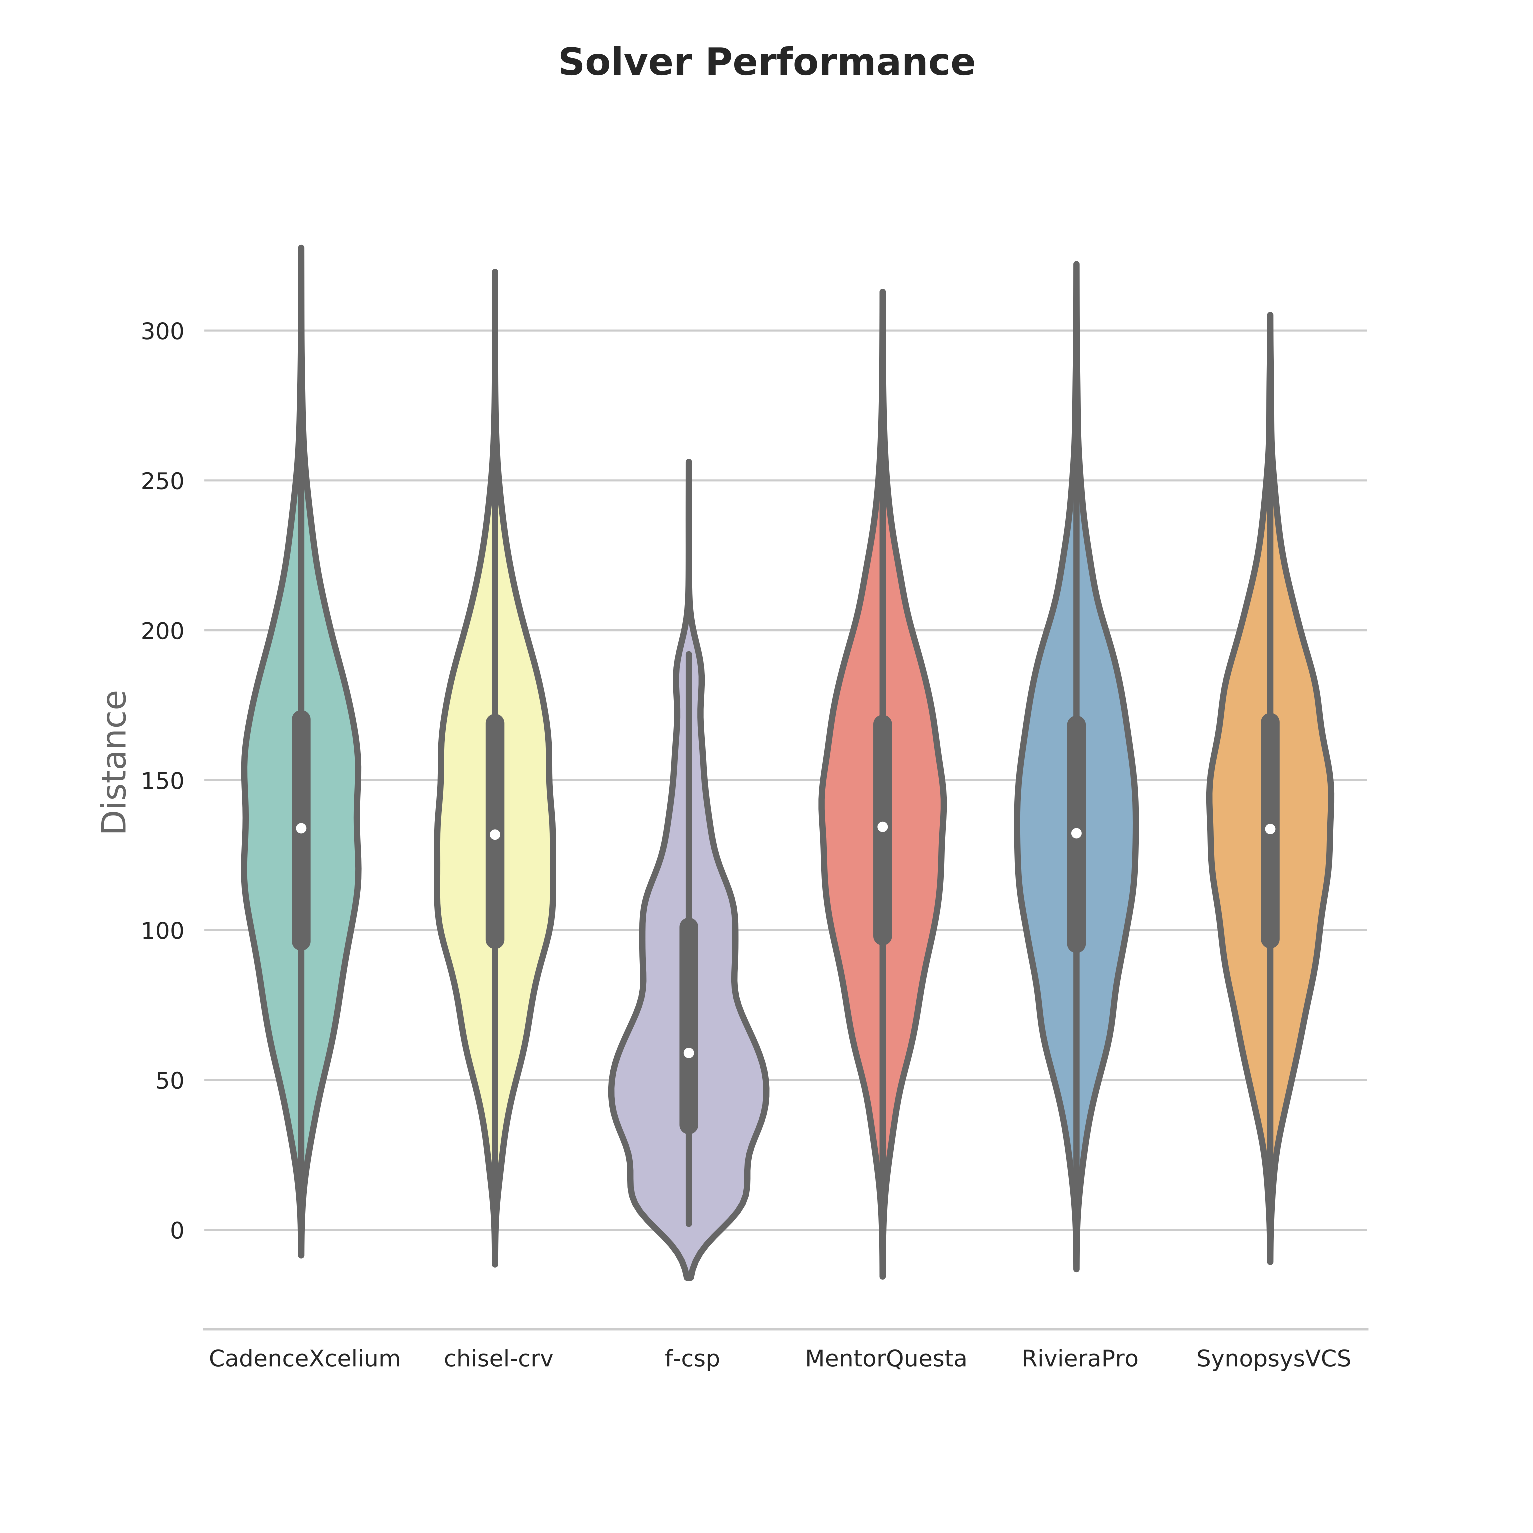
\includegraphics[width=0.7\linewidth]{pictures/Chisel-CRV_performance.eps}
\caption{Chisel-CRV evaluation.}
\label{fig:chiselcrv:distance}
\end{figure}

From picture \ref{fig:chiselcrv:distance}, it is clear that the JaCoP solver's
performances in this test are similar to the one provided by other commercial
solvers and significantly better than the F-CSP results.

\subsection{Comments about RandBundle}
Currently, random bundles are a feature marked experimental, and thus need to be
used carefully. The current implementation of \mints{RandBund} can automatically
infer the declared field's name in a \mints{Bundle} and generate a literal
\mints{Bundle}, but unfortunately, it cannot create a literal \mints{Bundle} if
it has nested \mints{Bundle}s or \mints{Vector}s as fields. This problem can be
circumvented by creating a method that returns the specific literal
\mints{Bundle} like in listing \ref{listing:crv:testinglit2}.

A second problem related to this implementation is the necessity of overriding
the \mints{typeEquivalent} field in the parent \mints{Bundle} definition to be
able to \mints{poke} and \mints{peek} the value of the generated \mints{Bundle}.
This overriding is necessary because ChiselTest performs a strict check of the
type equivalence before proceeding with the poke and peek during testing.

The main reason behind the limitations of \mints{RandBundle} class is related to
the fact that \mints{RandBundle} relies heavily on the Chisel library, while
\mints{RandObj} is a domain-specific language that lives in the Scala / Java
world. In version 3.2 of Chisel, an experimental package called
\mints{DataMirror} allowed the inspection the module ports and the retrieval of
some information about it like, their names, types, etc. Even with this set of
features introduced by the \mints{DataMirror} package, it is still not trivial
to create a complex literal \mints{Bundle} automatically at runtime.
